\section{Anforderungsanalyse}

Dieses Kapitel beschreibt die generellen Anforderungen an das Projekt, ohne auf Details wie die technische Machbarkeit ausführlich zu analysieren oder konkrete Umsetzungsstrategien zu planen. Diese softwaretechnischen Aspekte werden in Kapitel \ref{sec:implementation-analysis}~\nameref{sec:implementation-analysis} besprochen.

\info[inline]{Der Verzicht auf die technischen Hintergründe der Implementierung in diesem Kapitel soll es auch für ``normale'' Informatiklehrer verständlich machen, ohne Sie gleich mit den Details der Realisierung zu erschlagen.}

\subsection{Grundprinzipien}
\label{sec:principles}

Nach der Betrachtung der zu bedienenden Zielgruppe und der Beschäftigung mit bereits existierenden Alternativen, ist es nun an der Zeit ein paar allgemeine Grundprinzipien zu formulieren. Diese Prinzipien bilden die Philosophie hinter der Schülerentwicklungsumgebung ab und dienen als Leitfaden für Designentscheidungen.

Praktisch erlaubt das vor allem eine relativ akkurate Abschätzung, ob sich die Implementierung einer bestimmten Idee lohnt und wie sie zu priorisieren ist. Daher sind auch diese Prinzipien ihrer Bedeutung für diese Arbeit nach absteigend sortiert. Die sich dabei ergebende Auswahl berücksichtigt in den meisten Kapiteln auch den zur Verfügung stehenden Zeitrahmen der Masterthesis, ist also nicht nach rein didaktischen Gesichtspunkten zu bewerten.

\begin{description}
\item[Semantik vor Syntax] \hfill\\
  Den Lernenden sollen kontextsensitiv sinnvolle Operationen angeboten werden, optimalerweise mit einer kurzen Erläuterung, warum gerade nur diese Teilmenge an Operationen möglich ist. Die eigentliche Programmierung der Abfragen erfolgt dann durch die Kombination von Bausteinen, ähnlich wie bei der Lernsoftware ``Scratch''. Durch kontinuirliches Feedback der Entwicklungsumgebung sollen die Lernenden in die Lage versetzt werden, auch ohne eine ständige Rückversicherung bei der Lehrkraft die eigenen Ansätze zu erproben.
\item[Motivation durch praktisch vorzeigbare Ergebnissen] \hfill\\
  Typischerweise ist der Einstieg in die Programmierung von relativ langweiligen Programmen geprägt, häufig textbasierten Konsolenanwendungen. Im Sonderfall der Vermittlung von SQL Kenntnissen ist das Ergebnis der Arbeit sogar überhaupt nicht sinnvoll zu demonstrieren, weil die erstellten Abfragen isoliert für sich stehen und häufig auch nur in der Entwicklungsumgebung der jeweiligen Datenbank ausführbar sind. Mit der im Rahmen dieser Arbeit zu erstellenden Software sollen sich hingen praktisch relevante, allerdings sehr datenorientierte Programme umsetzen lassen. Diese verfügen über von den Lernenden zusammengestellte Eingabemasken um Daten einzufügen oder zu manipulieren und verschiedene Ausgabesichten um den Datenbestand sinnvoll zu präsentieren.
\item[Einfache Inbetriebnahme] \hfill \\
  Eine initiale Hürde jeder (Lern-)Software ist deren Installation, insbesondere bei Programmen aus dem Datenbankumfeld. Die Inbetriebnahme der für Server konzipierten Programme auf privaten, ``normalen'' Rechnern führt immer wieder zu Problemen aufgrund von nicht aufgelösten Abhängigkeiten oder fehlenden Rechten beim Starten von Systemdiensten oder bei Dateizugriffen. Die zunehmende Heterogenität an Betriebssystemen, insbesondere die zunehmende Verwendung MacOS, tut ein Übriges um die Verteilung von Software zu erschweren. Damit der eigentliche Lernprozess nicht schon vor dem Start der Entwicklungsumgebung behindert wird, hat eine möglichst einfache Inbetriebnahme dementsprechend Priorität. Prinzipiell stehen Informatiklehrkräfte bei dem Betrieb der jeweiligen Programme vor ähnlichen Problemen wie ihre Schüler, nur dass Sie auf die Konfiguration des Rechnerpools ihrer Schule oftmals nur einen eingeschränkten Einfluss haben. Die im Vergleich zu privaten Rechnern wesentlich restriktiver gehandhabte Rechte eines Schul-PCs verkomplizieren diesen Umstand zusätzlich.
\item[Schrittweise komplexere Benutzeroberfläche] \hfill \\
  Konventionelle Entwicklungsumgebungen sind Programme von Profis für Profis und bieten einen dementsprechend ausgerichteten Funktionsumfang. Gerade wenn man aber dabei ist etwas Neues zu lernen kann es sinnvoll sein, die Menge der möglichen Optionen zu beschränken. In diesem Sinne sollte auch die Lehrkraft die Möglichkeit haben den Funktionsumfang der Entwicklungsumgebung für Schüler gezielt zu reduzieren, falls einzelne Konzepte sich als noch zu fortgeschritten erweisen sollten.
\item[Fortführung der entwickelten Projekte] \hfill \\
  Viele Lernumgebungen sind in sich geschlossene Systeme, deren Arbeitsergebnisse nur schwer in anderen Programmen oder Kontexten von Nutzen sind. Sobald der Lernende dann die Grenzen der verwendeten Lernsoftware erreicht hat, steckt er in einer Sackgasse fest. Die Arbeitsergebnisse dieser zu entwickelnden Software sollen daher zumindest einfach einsehbar sein, optimalerweise nach einem Export sogar einfach mit gängigen externen Programmen erweiterbar.
  
  
\end{description}

\subsection{``Out-of-Scope''\todo{Deutsch?}}
\label{sec:out-of-scope}

Umgekehrt ist es auch wichtig, den Umfang des Projekts für die Thesis zu begrenzen. Die folgenden Ideen wären mehr oder minder naheliegende Ergänzungen, welche den Rahmen dieser Thesis aber sprengen würden.

\begin{description}
\item[Datenmodellierung] \hfill \\
  Der Schwerpunkt dieser Arbeit liegt zunächst auf der Vermittlung von Kenntnissen zur Abfrage und Manipulation von Daten in einem bestehenden Schema. Änderungen an diesem Schema sind nicht vorgesehen, demzufolge ist auch der Neuentwurf eines Schemas mit externen Mitteln zu bewerkstelligen. Völlig außerhalb des Umfangs dieser Arbeit ist die Überführung von konzeptionellen Modellen (z.B. ER-Schemata) in physikalische Modelle.
\item[Aufwändiges Design von Benutzerschnittstellen] \hfill \\
  Auch wenn die Konzeption der Benutzerschnittstelle für die verschiedenen Masken in den eben aufgezählten Prinzipien auftaucht, ist es wichtig den engen Rahmen dieses Aspektes zu verstehen. Es geht um die Schaffung von einfachen, datenzentrierten Eingabemöglichkeiten, nicht um die Umsetzung besonders kreativer Bedienkonzepte. Dementsprechend ist z.B. die Erweiterung der zur Verfügung stehenden Eingabeelemente durch die Lernenden außerhalb des Rahmens dieser Arbeit.
\end{description}

\subsection{Datenbanksystem}

Eine der naheliegendsten zu treffenden Entscheidungen hat zwar einen technischen Hintergrund, ist aber trotzdem unbedingt Bestandteil dieser Anforderungsanalyse: Es geht um die Wahl des zu lehrenden Datenbanksystems. Dieser Aspekt hat einen unmittelbaren Einfluss auf die Inbetriebnahme der Entwicklingsumgebung und auch auf die Fortführung der Projekte mit externen Programmen.

Im Hinblick auf die einfache Installation und Verwendung bietet sich eine eingebettete Datenbank an, da die Skalierung der von den Lernenden entwickelten Applikation vernachlässigt werden kann. Optimalerweise ist ein Backup des gesamten Datenbestandes mit einer einfachen Kopie einer Datei zu erledigen.

\unsure[inline]{Theoretisch ist die Menge an denkbaren Systemen fast unüberschaubar groß, praktisch sticht SQLite aus der Masse an Optionen heraus. Wie ausführlich muss ich das begründen?}

\subsection{Zwei Modi: Entwickeln und Anschauen}

Grundsätzlich unterschieden werden muss bei der Schülerentwicklungsumgebung, ähnlich wie bei Scratch, zwischen zwei Betriebsmodi für ein Projekt: Zunächst wird ein Projekt im Entwicklermodus betrieben, in diesem Fall stehen dem Benutzer alle Entwicklungstools zur Verfügung. Wenn es dann später einmal fertig ist und an Endanwender, z.B. Bekannte oder Freunde, weitergegeben wird, erwarte diese natürlich eine normale Benutzeroberfläche zu sehen. Der Wechsel zwischen diesen beiden Modi sollte dabei, ebenfalls analog zu Scratch, zu jedem Zeitpunkt möglich sein. Das ``Verstecken'' von Vorgehensweisen in Projekten ist also nicht vorgesehen. Im Endeffekt jedes Projekt auch als Vorlage für die Umsetzung eigener Ideen dienen können.

\subsection{Einfaches anlegen und kopieren von Projekten}

Im Sinne einer möglichst niedrigen Einstiegshürde soll es den Anwendern leicht gemacht werden, bestehende Projekte zu übernehmen. Im Informatikunterricht müssen häufiger zu Beginn bestimmte Schritte ausgeführt werden, ``weil das nun mal so'' (also eine ausführliche Erklärung zu diesem Zeitpunkt zu weit gehen würde). Im Falle des Sprachumfangs von SQL ist das zwar im Vergleich zu z.B. Java (``Herr Lehrer, was macht eigentlich dieses \texttt{public static void}?'') nicht ganz so dramatisch, aber nach Möglichkeit zu vermeiden.

Dementsprechend sollte möglichst jeder Schritt beim Anlegen eines neuen Projektes für die Schüler nachvollziehbar sein. Wenn dann doch einmal eine Serie von ``mechanisch auszuführenden'' Anweisungen erforderlich sein sollte, wäre es aber dennoch praktisch das durch eine Kopie eines schon bestehenden Projektes abzukürzen. Die Lehrkraft würde in diesem Fall also ein Projekt für ihre Schüler vorbereiten, welches diese dann optimalerweise mit einem einzigen Klick importieren können.

\subsection{Editor für SQL}
\label{sec:design-sql-editor}

Der grafische Editor soll grundsätzlich ähnlich zu den aus Scratch bekannten Bedienkonzepten funktionieren. Es kommen also distinkte Bedienelemente für die verschiedenen Komponenten einer SQL Abfrage zum Einsatz, kein reiner Texteditor. Der komponentenorientierte Editor soll dabei nicht unbedingt die Konzeption von beliebigen Abfragen ermöglichen, wohl aber die in Kapitel \ref{sec:example-queries} \nameref{sec:example-queries} beschriebenen exemplarischen Arbeitsabläufe unterstützen. 

Wenn ein Anwender der Entwicklungsumgebung an die Grenzen des unterstützenden Editors stößt, sollte er die Möglichkeit haben einmalig und für diese konkrete Abfrage eine Umwandlung in eine textbasierte Darstellung vornehmen zu können. Der umgekehrte Weg, also der Import von beliebigen SQL-Abfragen in den grafischen Editor, ist jedoch explizit ausgeschlossen.

Grundsätzlich bedürfen einige Komponenten der Abfrage besonderer Aufmerksamkeit, weil sie große Auswirkungen auf das Verhalten der anderer Komponenten haben. Vorrangig ist hier die \texttt{GROUP-BY} Komponente zu nennen. Sobald die Query mit einer \texttt{GROUP BY} Komponente ausgestattet wird ist der Zugriff auf die konkreten Spalten einzelner Zeilen z.B. im allgemeinen Fall nicht mehr möglich. Das hinzufügen (oder entfernen) dieser Komponente hat also große Auswirkungen auf die Korrektheit der gesamten Abfrage.

\subsubsection{Visuelle Gestaltung}

Für technische Details irrelevant, aber unbedingt ebenfalls im Voraus zu klären ist die Frage, ob es sinnvoll wäre, das sehr bunte, blockige Design von Scratch zu imitieren. Abbildung \ref{fig:compare-colourful} zeigt einen Vergleich eines frühen Prototypen in einem an Syntax-Highlighting angelehnten Design und in einem wesentlich bunteren, blockigen Design.

\todo[inline]{\textbf{Todo}: Quelle mit Beleg für ``Kinderfreundliches'' buntes Design suchen. Das wird man bei Scratch schon aus gutem Grund gemacht haben. Relevante Frage: Zielgruppe (in Jahren) von Scratch vs. Zielgruppe dieses Projektes?}

Aber auch wenn man den sehr bunten Stil gegen einen etwas nüchtereren, aber immer noch ``blockartigen'' Stil austauschen würde, ergeben sich dadurch nur vergleichsweise wenige Vorteile. In Scratch zeigen z.B. die Konnektoren des Blocks für eine Endlosschleife sehr deutlich, wie sich der Kontrollfluss durch dieses Element verändern wird. Für eine vollständige Programmiersprache ist das mit Sicherheit eine gute Wahl, aber für den sehr linearen Ablauf einer SQL-Abfrage ist dieser Umstand nicht von Bedeutung.

Ein weiterer Vorteil eines etwas nüchterneren, IDE-ähnlichen Designs wäre zudem die größere Nähe zu ``normalen'' Entwicklerprogrammen. Diese wirken möglicherweise weniger einschüchternd, wenn man sich schon an den Anblick von recht viel Text mit Syntax-Highlighting gewöhnt hat.

Letztendlich überwiegt aber ein sehr viel profanerer Fakt: Der Autor dieser Arbeit ist kein Grafikdesigner und würde vermutlich kein ansprechendes und zugleich buntes Farbkonzept auf die Beine stellen können.

\begin{figure}
  \begin{subfigure}[b]{0.45\textwidth}
    \includegraphics[width=\textwidth]{images/sql-sketch-early-colourful}
    \caption{Starke Farbakzente, ähnlich zu Scratch}
    \label{fig:screen-sql-editor-early-colourful}
  \end{subfigure}\hfill
  \begin{subfigure}[b]{0.45\textwidth}
    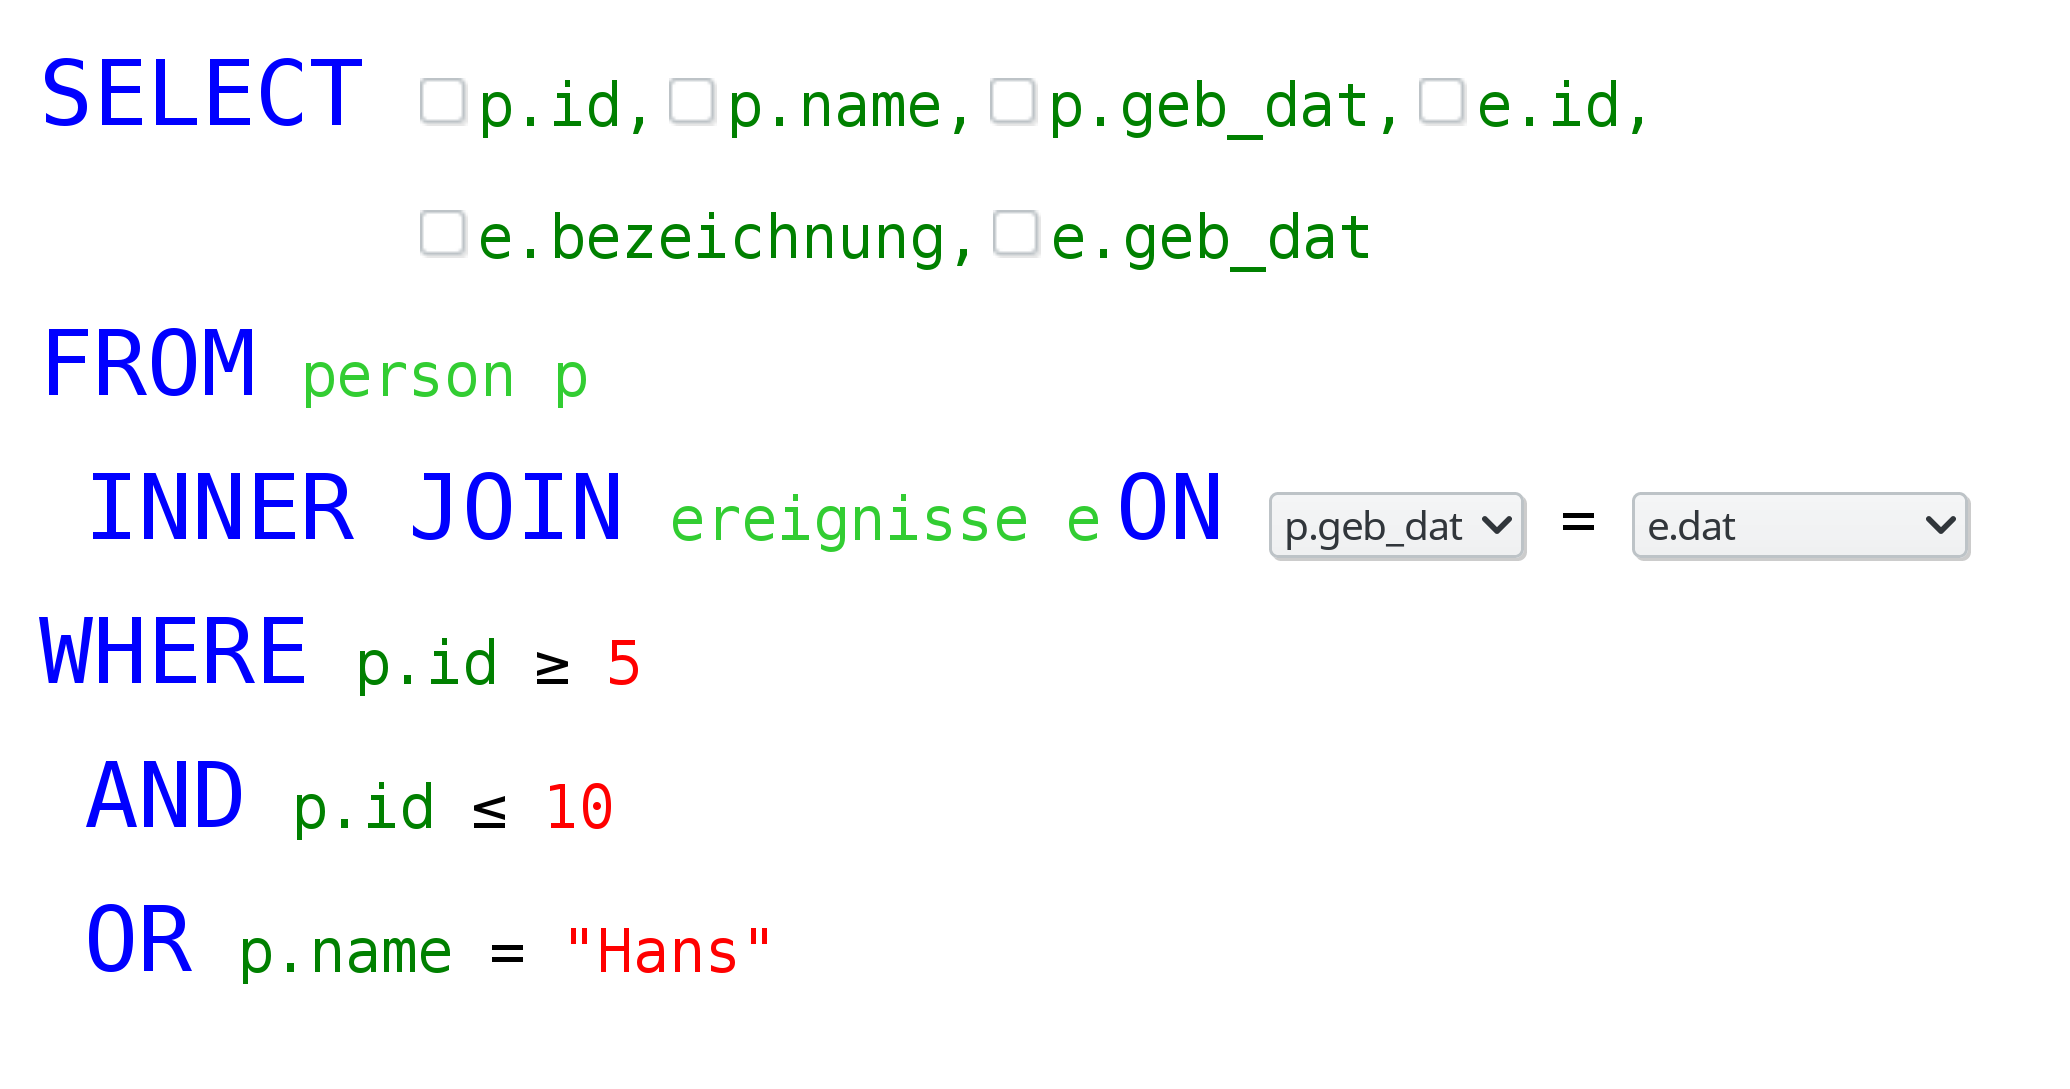
\includegraphics[width=\textwidth]{images/sql-sketch-early-syntax-highlight}
    \caption{Syntax-Highlighting, ähnlich einer IDE}
    \label{fig:screen-sql-editor-early-syntax-highlighting}
  \end{subfigure}
  \caption{Vergleich unterschiedlicher Gestaltungsansätze}
  \label{fig:compare-colourful}
\end{figure}

\subsubsection{Grundsätzlicher Aufbau des Editors}

Ein grundsätzlicher Nachteil dieses Komponentenorientierten Bedienkonzeptes ist der nötige Platz für die Unterbringung aller verwendbaren Komponenten. Es muss sorgfältig geplant werden, wie diese anzuordnen sind und welche Optionen in welchem Kontext gerade sichtbar sein müssen. Anders als bei Scratch muss dabei nicht unbedingt Drag \& Drop das vorherrschende Bedienparadigma sein. Da der Benutzer immer nur eine Abfrage zur Zeit bearbeiten können soll, ergibt sich der einzig mögliche Platz für viele Blöcke automatisch. Darüber hinaus ist die Reihenfolge eines Großteils der Komponenten einer Abfrage sehr strikt festgelegt, so kann eine \texttt{GROUP BY} Komponente nicht an beliebigen Stellen verwendet werden, sondern nur nach der \texttt{FROM} oder der \texttt{WHERE} Anweisung. Andere Komponenten wie z.B. \texttt{HAVING} oder logische Verknüpfungen mit \texttt{AND} oder \texttt{OR} sind nicht nur von der Reihenfolge, sondern auch von der Existenz anderer Bestandteile abhängig. Die Verwendung eines separaten Bereichs mit allen Bestandteilen einer SQL-Abfrage (bei Scratch ``Toolbox'' genannt) wäre also zwar denkbar, sollte aber zumindest keinesfalls Drag \& Drop erzwingen, sofern das hinzufügen der Komponente nur an einer einzigen Stelle möglich ist.

\begin{wrapfigure}{r}{0.46\textwidth}
  \includegraphics[width=0.45\textwidth]{images/sql-sketch-all-editing}
  \caption{So nicht! Simultane Anzeige (fast) aller Möglichkeiten}
  \label{fig:screen-sql-editor-all-editing}
\end{wrapfigure}

Die Alternative dazu wäre eine Anzeige von ``Platzhaltern'' für die entsprechenden Komponenten unterhalb der eigenen Abfrage. Ein Klick auf den Platzhalter wandelt diesen dann in einen konkreten Block um und fordert ggfs. zur Angabe der benötigten Parameter auf. Im Rahmen der entwickelten Prototypen hat sich herausgestellt, dass eine permanente Anzeige aller Editierungsmöglichkeiten mit einem sehr überladen wirkenden Benutzerinterface einher geht, insbesondere was die Einblendung von Platzhaltern angeht. Abbildung \ref{fig:screen-sql-editor-all-editing} zeigt einen Screenshot des Prototypen, bei dem nahezu alle denkbaren Editierungsoptionen gleichzeitig verfügbar sind.

Dementsprechend wird ein anderer Ansatz verfolgt werden müssen: Es lässt sich immer ein Block zur Zeit in einen ``editieren'' Modus versetzen. Nur innerhalb dieses Blocks erlauben die Bedienelemente dann eine Änderung der Komponente. Für einige Komponenten, speziell \texttt{FROM}, \texttt{WHERE} und \texttt{HAVING} lassen sich neu anzuhängende Komponenten auch sehr gut im Rahmen dieses Modus anbieten. Es stellt sich dann natürlich die Frage, wie man Blöcke ohne einen eindeutig passenden Kontext, z.B. ein \texttt{ORDER BY}, der Abfrage hinzufügen kann. Eine Antwort darauf wird sich vermutlich erst durch reale Tests mit der Oberfläche finden lassen, die folgenden Ansätze sind aber denkbar:

\begin{itemize}
  \item Die \texttt{SELECT}-Komponente hat einen losen Bezug zu allen anderen Komponenten. Schwierig einzuordnende Komponenten wie \texttt{WHERE}, \texttt{GROUP BY}, \texttt{ORDER BY} \texttt{LIMIT} oder auch \texttt{UNION} werden immer dann angeboten, wenn die \texttt{SELECT}-Komponente gerade editiert wird.
  \item Eine Leiste mit möglichen Komponenten ohne eindeutigen Kontext erlaubt deren Ergänzung zu jedem Zeitpunkt.
\end{itemize}

\info[inline]{Im Editor immer zu sehen, aber aktuell nicht beschrieben: Eine Tabelle mit den Daten, welche die Abfrage im aktuellen Zustand liefern würde.}

\subsubsection{Vergleiche und Ausdrücke}
\label{sec:sql-compare-and-expression}

Die Abbildungen des Prototypen haben einen Umstand schon vorweggenommen: Die Vergleiche in den \texttt{ON} und \texttt{WHERE} Ausdrücken sollten nach Möglichkeit keine einfachen Textfelder sein, sondern dem Benutzer sinnvolle, kontextabhängige Vorschläge machen.

Da es an allen Stellen, bei denen in SQL Werte verglichen oder ausgegeben werden, möglich ist, diese durch Funktionen zu verändern oder durch Ausdrücke zu berechnen, wird allerdings ein Rückgriff auf freie Ausdrücke vorgesehen werden müssen. Es wird kaum möglich sein, einen gestützten Editor für den vollen Umfang aller denkbaren Funktionen bereitzustellen: spätestens aufgrund der möglichen Schachtelung von Ausdrücke können diese sehr schnell enorm kompliziert werden. Eine inhaltliche Prüfung dieser Ausdrücke ist zumindest im Rahmen dieser Arbeit nicht zu leisten.

Und trotzdem lässt sich ein Großteil der für die Schüler nötigen Verknüpfungen oder Ausdrückeganz gut kontextgestützt implementieren. Dieser Unterstützungsprozess basiert dabei auf Datentypen und geht immer von der Auswahl einer Spalte der Abfrage aus. Wenn ein Schüler also einen neuen Vergleich hinzufügen möchte, wählt er zunächst eine Spalte und erhält dann Vorschläge für mögliche Operatoren und die rechte Seite des Vergleichs. Für Ausdrücke im \texttt{SELECT} ist dieses Vorgehen ähnlich, das Ergebnis des Ausdrucks muss dann nur nicht zwingend ein Boolescher Wert sein.

\begin{itemize}
\item Für \texttt{TEXT} Spalten können in Ausdrücken einige einfache Stringfunktionen wie \texttt{LOWER} oder \texttt{UPPER}) angeboten werden. Ebenfalls interessant wäre eine Implementierung der \texttt{LENGTH}-Funktion, da diese einen vom Parametertyp abweichenden Rückgabetyp aufweist.
\item Mathematische Ausdrücke für \texttt{NUMBER} Spalten sind ebenfalls denkbar, der nötige Implementierungsaufwand ist im Vergleich zum erwartbaren Nutzen allerdings vergleichsweise groß.
\item Im Falle des Vergleichs von \texttt{NUMBER} Spalten werden konstante Werte oder andere \texttt{NUMBER} Spalten angeboten.
\item Für Vergleiche von \texttt{TEXT} Spalten bietet sich der unscharfe Vergleich mit dem \texttt{LIKE} Ausdruck an.
\item Perspektivisch interessant, aber vermutlich schon außerhalb des Umfangs dieser Arbeit, wäre der Umgang mit Datums und Zeitfunktionen.
\end{itemize}

\unsure[inline]{Ich bin mir noch nicht sicher, wie ich das gerne handhaben möchte. Vermutlich ein mehr oder minder separater Editor für Ausdrücke? Auf jeden Fall muss ich hier den Umfang sehr deutlich vorher abstecken. Gerade an dieser Stelle wäre ein Scratch-ähnlicher Editor dann doch wieder ein echter Gewinn. Für den Anfang wird es aber auch ein einfaches Textfeld tun müssen, von da aus kann ich dann schauen wie weit ich komme.}

\subsubsection{\texttt{GROUP BY}}

Sobald in einer Abfrage eine \texttt{GROUP BY} Komponente auftaucht, hat dies Auswirkungen auf die Möglichkeiten innerhalb der \texttt{SELECT} Anweisung. Da keine Auswahl von ungruppierten und nicht-aggregierten Spalten möglich sein darf, müssen diese entfernt werden. Insbesondere wenn der Benutzer vorher schon mit komplizierten Ausdrücken im \texttt{SELECT} gearbeitet haben sollte, ist also zumindest eine Warnung nötig.

Danach verhält es sich mit den Aggregatsfunktionen nicht anders als mit den im vorigen Abschnitt beschriebenen Vergleichen und Ausdrücken, nur dass halt in diesem Kontext andere Funktionen zur Verfügung stehen.

\subsubsection{Verknüpfungen mit \texttt{JOIN}}

Sofern ein Editor für Ausdrücke (siehe \ref{sec:sql-compare-and-expression}) vorausgesetzt werden kann, lassen sich Verknüpfungen ohne größeren Mehraufwand fast vollumfänglich umsetzen. Im Falle von \texttt{JOIN}-Ausdrücken mit \texttt{USING} wird sich im Regelfall sogar exakt eine Spalte für die Verknüpfung anbieten. Bei Ausdrücken mit \texttt{ON} muss dann der Rückgriff auf den Editor für Ausdrücke erfolgen.

\subsubsection{Deaktivierbare Komponenten}

Unmittelbar nach dem Hinzufügen einer neuen Komponente sind möglicherweise noch nicht alle nötigen Informationen verfügbar. Daher werden Komponenten immer in einem deaktivierten Zustand hinzugefügt, sie lassen sich erst aktivieren wenn alle relevanten Informationen eingetragen worden sind. Genau so werden Komponenten mit inhaltlichen Fehlern deaktiviert, bis der Fehler behoben worden ist. Und natürlich kann es auch Gründe geben eine Komponente freiwillig zu deaktivieren, auch das soll selbstverständlich möglich sein.

Speziell für die \texttt{WHERE} und \texttt{HAVING} Komponenten ist zu klären, welche Auswirkung eine Deaktivierung haben soll. Sollen alle Kinder ebenfalls deaktiviert werden oder wird die nächste folgende Komponente zum \texttt{WHERE} bzw. \texttt{HAVING}? Auch hier sind beide Möglichkeiten denkbar, die bessere Alternative muss sich durch Tests mit realen Benutzern zeigen.

\subsubsection{Änderung der Reihenfolge}

Wiederum für die \texttt{WHERE} und \texttt{HAVING}, aber auch für die \texttt{JOIN} Komponenten wäre es sehr hilfreich, die Reihenfolge durch eine Schaltfläche oder auch Drag \& Drop variieren zu können.

\subsubsection{Unterabfragen}

Noch komplizierter wird der Umgang mit Ausdrücken, wenn man in diesen auch Unterabfragen zulassen möchte.

\unsure[inline]{Hier das gleiche Problem wie mit Ausdrücke, ich tendiere momentan zu ``mach ich nicht, sehe ich wenn überhaupt konzeptuell vor''.}

\subsubsection{Abfragen mit Parametern}
\label{sec:design-query-params}

Um eine Interaktion mit Endbenutzern zu ermöglichen können in Abfragen auch benannte Parameter anstelle von konstanten Werten verwendet werden. Diese müssen dann zur Laufzeit vom Benutzer angegeben werden. Aus Sicht der SQL-Abfrage ist diese Ergänzung relativ trivial, die eigentliche Problematik liegt im Binden dieser Parameter zur Laufzeit. Das Kapitel \ref{sec:design-ui-editor} beschreibt den Editor für Benutzeroberflächen, durch welchen die Verknüpfung mit den Bedienelementen der Oberfläche vorgenommen wird.

\subsubsection{Manipulation von Daten}

Neben den bisher ausführlich besprochenen \texttt{SELECT}-Anweisungen müssen sich natürlich \texttt{INSERT}-, \texttt{UPDATE}- und \texttt{DELETE}-Anweisungen umsetzen lassen. Da diese ihrer Natur nach nicht idempotent sind verbietet sich natürlich eine wiederholte, automatische Ausführung während der Entwicklungszeit. Es ist zu erwarten, dass die meisten von den Schülern verfassten Abfragen ausführlichen Gebrauch von den in Kapitel \ref{sec:design-query-params} beschriebenen Parametern machen.

\subsection{Didaktisch sinvolle Teilmengen von SQL}
\label{sec:sql-subset}

Das vorige Kapitel hat schon viele praktische Probleme bei einer uneingeschränkten Umsetzung des SQL-Standards aufgezeigt und dabei wiederholt von einer nicht näher definierten ``sinnvollen Teilmenge'' gesprochen. Genau diese Definition wird nun in diesem Kapitel nachgeholt.

\subsubsection{Mögliche lokale Einschränkungen}
\label{sec:sql-subset-local}

\warning{Nicht alle hier beschriebenen Optionen sind notwendigerweise in der Entwicklungsumbegung implementiert! Dieses Kapitel ist eine \textit{allgemeine} Betrachtung von didaktisch sinnvollen Teilmengen von SQL. Um zu sehen, welche Funktionalität tatsächlich implemtiert worden ist lohnt sich ein Blick in Anhang \ref{app:implemented-features}:~\nameref{app:implemented-features}.}

Wir klären in diesem Kapitel zunächst, welche Features von SQL überhaupt für die Entwicklungsumgebung von Belang sind und wie diese voneinander abhängen. Die Abgrenzung von Teilsprachen baut auf diesen hier herausgearbeiteten Optionen auf und ist Gegenstand von Kapitel \ref{sec:sql-subset-ranks}.

Glücklicherweise erlaubt die Struktur von SQL die Angabe von sehr lokalen Einschränkungen, deren Auswirkungen sich sehr gut abschätzen lassen. Einzig der Umgang mit Ausdrücken überspannt viele Bereiche von SQL: Diese können an sehr vielen Stellen auftreten und müssen dementsprechend sorgfältig analysiert werden. Daher beschränken sich alle Stellen an denen der Einsatz von Ausdrücken sinnvoll möglich ist auf eine einfache ``Ausdrücke zulassen'' Option, deren Details dann später separat geregelt werden.

\unsure[inline]{Erwähnen, inwiefern das herauslösen von Sprachfeatures bei einer ``normalen'' Programmiersprache komplizierter wäre? Es gibt bei SQL halt vergleichsweise wenige Abhängigkeiten und daher viele mögliche Reihenfolgen in denen man die Features aktivieren kann. Bei einer Sprache wie z.B. Java bauen die einzelnen Sprachfeatures sehr viel stärker aufeinander auf, es ergeben sich deutlich weniger Reihenfolgen in denen man diese sinnvoll aktivieren könnte.}

Technisch gesehen soll es für Lehrkräfte möglich sein, fast beliebige Teilmengen von SQL für ihre Schüler vorzugeben, nicht nur die im Rahmen dieser Arbeit als sinnvoll erachteten Kombinationen. Das grundsätzliche Vorgehen sollte dabei einer Whitelist entsprechen: Jede explizit erlaubte Funktionalität steht im SQL-Editor (siehe \ref{sec:design-sql-editor}) zur Verfügung. Und sofern eine Funktionalität nicht erlaubt sein sollte, ist sie auch nicht verfügbar.

Prinzipiell wäre es auch denkbar, in unterschiedlichen Komponenten verschiedene Teilmengen der Ausdrücke zuzulassen, inhaltlich erscheint das aber wenig sinnvoll. Die Schüler sollen durchaus verstehen, dass es sich bei Ausdrücken in SQL um ein allgemeines Konzept handelt, welches Prinzipiell in der \texttt{SELECT}-Komponente genau so angewandt werden kann wie beim \texttt{ORDER BY}. Das folgende Beispiel erklärt den Gedankengang dahinter etwas griffiger: Wenn sich die Schüler aus didaktischen Gründen erstmal nur mit Ausdrücke im Rahmen der \texttt{SELECT}-Komponente beschäftigen sollen ist das eine sinnvolle, und daher mögliche Einschränkung. Nicht sinnvoll hingegen wäre es die Anwendung der \texttt{LENGTH(X)} Funktion nur in einer der beiden Komponenten zuzulassen. Letzteres wird daher auch nicht unterstützt.

Einige der hier beschriebenen Optionen sind redundant. Das liegt zum einen an SQL selbst, die Sprache sieht schlichtweg mehrere syntaktische Varianten für semantisch äquivalente Sachverhalte vor. Zum anderen kann es aber auch aus didaktischen Gründen sinnvoll sein, die Wissensvermittlung mit einer Reihe von Spezialfällen zu beginnen\todo{Beleg}.

\begin{enumerate}
\item \textbf{Projektionen mit \texttt{SELECT}} \\
  Diese Komponente als solche kann natürlich nicht ausgeschlossen werden. Außerdem muss mindestens \ref{feat:select-all} $\lor$ \ref{feat:select-column} erlaubt sein, sonst können keine gültigen SQL-Abfragen erstellt werden.
  \begin{enumerate}
  \item \label{feat:select-all} Auswahl aller Spalten (``Sternchen-Operator'' \texttt{SELECT *})
  \item \label{feat:select-column} Auswahl von Spalten
  \item \label{feat:select-alias} Vergabe von Aliasnamen
  \item \label{feat:select-expression} Anwendung von Ausdrücken
  \item \label{feat:select-sub} Unterabfragen in Ausdrücken zulassen
  \end{enumerate}
\item \textbf{Angabe von Datenquellen mit \texttt{FROM}} \\
  Auch die Auslassung dieser Komponente ist nicht zulässig, obwohl einige SQL Dialekte dies durchaus erlauben. Der Mehrwert dieser Auslassung wäre aus didaktischer Sicht aber nicht gegeben: Die Schüler sollen SQL Abfragen grundsätzlich auf Tabellen beziehen und keine Daten ``aus der Luft greifen''. Die Funktionalität der komplexen \texttt{ON}-Bedingung \ref{feat:from-on-expression} hängt von den Möglichkeiten im \texttt{WHERE} und \texttt{HAVING} ab.
  \begin{enumerate}
  \item \label{feat:from-cross-join} Kreuzprodukt (\texttt{JOIN}) zulassen
  \item \label{feat:from-cross-comma} Kreuzprodukt (komma-separierte Schreibweise) zulassen
  \item \label{feat:from-natural-join} Automatische innere Verknüpfung zulassen (\texttt{NATURAL JOIN})
  \item \label{feat:from-inner-join} Innere Verknüpfung zulassen (\texttt{INNER JOIN}), erfordert \ref{feat:from-using} $\lor$ \ref{feat:from-on-simple} $\lor$ \ref{feat:from-on-expression}
  \item \label{feat:from-left-join} Linke äußere Verknüpfung zulassen (\texttt{LEFT OUTER JOIN}), \ref{feat:from-using} $\lor$ \ref{feat:from-on-simple} $\lor$ \ref{feat:from-on-expression}
  \item \label{feat:from-right-join} Rechte äußere Verknüpfung zulassen (\texttt{RIGHT OUTER JOIN}), \ref{feat:from-using} $\lor$ \ref{feat:from-on-simple} $\lor$ \ref{feat:from-on-expression}
  \item \label{feat:from-full-join} Volle äußere Verknüpfung zulassen (\texttt{FULL OUTER JOIN}), \ref{feat:from-using} $\lor$ \ref{feat:from-on-simple} $\lor$ \ref{feat:from-on-expression}
  \item \label{feat:from-using} \texttt{USING}-Bedingung zulassen
  \item \label{feat:from-on-simple} Einfache \texttt{ON}-Bedingung mit Vergleichsoperator zulassen
  \item \label{feat:from-on-expression} Allgemeine Ausdrücke in \texttt{ON}-Bedingung zulassen
  \item \label{feat:from-recursive} Rekursive Verknüpfung zulassen 
  \item \label{feat:from-sub} Unterabfragen zulassen
  \end{enumerate}
\item \textbf{Filterung mit \texttt{WHERE} und \texttt{HAVING}} \\
  Da an dieser Stelle Ausdrücke zum Einsatz kommen, sind prinzipiell zwei unterschiedliche Ansätze denkbar. Zunächst ist es möglich eine Reihe von ``typischen'' Vergleichen zuzulassen. Die Optionen \ref{feat:where-compare-const}, \ref{feat:where-compare-null}, \ref{feat:where-compare-other-col}, \ref{feat:where-compare-simple-func}, \ref{feat:where-compare-simple-expression} und \ref{feat:where-compare-negate} sind nichts weiter als eine Aneinanderreihung von speziellen Vergleichen, mit denen sich aber der Großteil aller Einschränkungen vornehmen lassen können sollte. Dem gegenüber steht der Ansatz einfach beliebige boolesche Ausdrücke zu erlauben, was sowohl die Komplexität der möglichen Ausdrücke steigert als auch den Anspruch an den Benutzer erhöht.
  \begin{enumerate}
  \item \label{feat:where-allow} \texttt{WHERE} zulassen
  \item \label{feat:having-allow} \texttt{HAVING} zulassen
  \item \label{feat:where-and} Verknüpfungen mit \texttt{AND}
  \item \label{feat:where-or} Verknüpfungen mit \texttt{OR}
  \item \label{feat:where-compare-const} Vergleich einer Spalte der Ergebnismenge mit einem konstanten Wert
  \item \label{feat:where-compare-null} Vergleich einer Spalte der Ergebnismenge gegen \texttt{NULL}
  \item \label{feat:where-compare-other-col} Vergleich einer Spalte der Ergebnismenge mit einer anderen Spalte der Ergebnismenge
  \item \label{feat:where-compare-simple-func} Vergleich einer Spalte der Ergebnismenge mit einem einfachen (nicht geschachtelten) Funktionsausdruck
  \item \label{feat:where-compare-simple-expression} Vergleich einer Spalte der Ergebnismenge mit einem einfachen Rechenausdruck
  \item \label{feat:where-compare-negate} Negation simpler Ausdrücke
  \item \label{feat:where-any-expression} Beliebige Vergleichsausdrücke, also keine strukturelle Einschränkung der Vergleiche
  \item \label{feat:where-like} Nutzung des \texttt{LIKE}-Operators
  \item \label{feat:where-between} Nutzung des \texttt{BETWEEN}-Operators
  \item \label{feat:where-in} Nutzung des \texttt{IN}-Operators

    \unsure[inline]{Umgang mit Platzhaltern}
  \end{enumerate}
\item \textbf{Bildung von Gruppen mit \texttt{GROUP BY}}
  \begin{enumerate}
  \item \label{feat:group-allow} \texttt{GROUP BY} zulassen
  \item \label{feat:group-multiple} Grupperierung mehrerer Spalten zulassen
  \end{enumerate}
\item \textbf{Sortierung mit \texttt{ORDER BY}} \\
  Bei dieser Komponente fehlt bewusst die Möglichkeit anhand eines Spaltenindexes aus dem \texttt{SELECT} zu sortieren. Da die gute Lesbarkeit der Abfragen ein erklärtes Ziel der Entwicklungsumgebung ist, wurde auf diese redundante Möglichkeit der Spaltenauswahl verzichtet.
  \begin{enumerate}
  \item \label{feat:order-allow} \texttt{ORDER BY} zulassen, die Auswahl der Richtung (\texttt{ASC} und \text{DESC}) ist dann grundsätzlich möglich
  \item \label{feat:order-select} Sortierung nach im \texttt{SELECT} erwähnten Spalten oder Ausdrücken zulassen
  \item \label{feat:order-any-column} Sortierung nach beliebigen Spalten zulassen
  \item \label{feat:order-expression} Sortierung anhand eines beliebigen Ausdrucks zulassen
    \unsure[inline]{Umgang mit Platzhaltern}
  \end{enumerate}
  
  \begin{enumerate}
  \item \textbf{Beschränkung der Datenmenge mit \texttt{LIMIT}} \\  
    \unsure[inline]{Vermutlich nötig für Oberfläche}
  \end{enumerate}
\end{enumerate}

Nach dieser Betrachtung der mit der unmittelbaren SQL-Syntax zusammenhängenden Funktionalität ist es nun an der Zeit, sich den Ausdrücken ausführlicher zu widmen.

\begin{enumerate}
\item \textbf{Allgemeine Funktionen (in alphabetischer Reihenfolge)} \\
  In einem Umfeld für Anfänger ist zu erwarten, dass fast jede Funktion (bzw. jede logische Gruppe an Funktionen) einer eigenen Einführung bedarf. Die Lehrkräfte sollen diese daher isoliert zur Verfügung stellen können, ohne Ablenkung durch nicht benötigte Funktionen. Ferner werden verschiedene Variante der gleichen Funktionen vermieden, um Irritationen zu vermeiden.
  \begin{enumerate}
  \item \label{feat:fun-abs} \texttt{ABS(X)}
  \item \label{feat:fun-coalesce} \texttt{COALESCE(X,Y,...)}
  \item \label{feat:fun-length} \texttt{LENGTH(X)}
  \item \label{feat:fun-casing} \texttt{LOWER(X)} und \texttt{UPPER(X)}
  \item \label{feat:fun-random} \texttt{RANDOM()}
  \item \label{feat:fun-round} \texttt{ROUND(X,Y)}
  \item \label{feat:fun-trim} \texttt{TRIM(X)} sowie \texttt{LTRIM(X)} und \texttt{RTRIM(X)}
  \end{enumerate}

\item \textbf{Aggregierende Funktionen (in alphabetischer Reihenfolge)} \\
  Die Verfügbarkeit dieser Funktionen hängt von der Verfügbarkeit der \texttt{GROUP BY}-Komponente ab (\ref{feat:group-allow}).
  \begin{enumerate}
  \item \label{feat:fun-avg} \texttt{AVG(X)}
  \item \label{feat:fun-count} \texttt{COUNT(X)}
  \item \label{feat:fun-group-concat} \texttt{GROUP\_CONCAT(X,Y)}
  \item \label{feat:fun-max-min} \texttt{MAX(X)} und \texttt{MIN(X)}
  \item \label{feat:fun-sum} \texttt{SUM(X)}, gibt im Falle von komplett fehlenden Werten \texttt{NULL} zurück
  \item \label{feat:fun-total} \texttt{TOTAL(X)}, gibt im Falle von komplett fehlenden Werten \texttt{0.0} zurück
  \end{enumerate}
\end{enumerate}

\subsubsection{Sprachstufen}
\label{sec:sql-subset-ranks}

Angelehnt an die bei Racket genutzte Idee der Feature-Levels soll dieses Kapitel einige sinnvolle Untermengen von SQL definieren, auf denen die mitgelieferten Beispielprojekte aufbauen. Es handelt sich dabei um Vorschläge, nicht um die einzig möglichen Ausprägungen von sinnvoll reduzierten SQL-Varianten.

\missing[inline]{Ich muss erst noch ein paar mehr Beispiele an der Hand haben, bis ich mich diesem Kapitel erneut widme.}

\subsection{Konzept für Oberflächen}
\label{sec:design-ui-editor}

Damit sich mit der Schülerentwicklungsumgebung erstellte Projekte auch von normalen Endanwendern bedienen lassen können Bedarf es natürlich einer entsprechenden Benutzeroberfläche. Hier bietet sich aus Gründen der einfachen Weitergabe eine webbasierte Oberfläche an: So entfällt bei den Endanwendern jegliche Installation und gerade für datenzentrierte, verteilte Anwendungen ist eine einheitliche Sicht auf den Datenbestand selbstverständlich essentiell. Beides Umstände, die sich gut mit einem zentralen Datenbestand auf einem Server erreichen lassen.

Diese Oberflächen werden in HTML mit einigen Erweiterungen durch Angular 2 definiert, was vor den Anwendern der Schülerentwicklungsumgebung allerdings verborgen wird. Ähnlich wie für die SQL Abfragen ist also auch für diese Oberflächen ein dezidierter Editor zu implementieren. Die Schüler sollten zu keinem Zeitpunkt selber HTML-Code schreiben müssen, optional aber durchaus die Möglichkeit dazu haben.

\subsubsection{Bedienelemente ohne Bindung an Daten}

Zwar sollen im Regelfall keine komplett statischen Seiten angezeigt werden, trotzdem muss es natürlich eine Möglichkeit geben statische Texte ohne Bindung an irgendwelche Abfragen zur Anzeige zu bringen.

\begin{description}
  \item[Überschriften] \hfill \\
    HTML sieht die Verwendung von Überschriften in sechs Hierarchiebenen vor und stellt dafür distinkte Elemente zur Verfügung (\texttt{<h1>} bis \texttt{<h6>}). Dieser Umstand soll nicht unmittelbar im Bedienkonzept des Editors abgebildet werden: Hier soll es das allgemeine Bedienelement ``Überschrift'' geben, zu dem sich dann eine Ebene auswählen lässt.
  \item[Absätze] \hfill \\
    Blöcke von zusammenhängendem Text werden als Absatz ausgezeichnet, das entsprechende HTML-Äquivalent ist das \texttt{<p>}-Element.
  \item[Listen] \hfill \\
    Strukturiert zusammenhängende Daten werden als sortierte oder unsortierte Liste (\texttt{<ol>} bzw. \texttt{<ul>} in HTML) gruppiert.
      
\end{description}

\subsubsection{Bindung von Daten an die Oberfläche}

Ein Großteil der Oberflächenelemente wird einige Eigenschaften aufweisen, deren Inhalte erst zur Laufzeit dynamisch gebunden werden. Dabei stellt sich die Frage, wie die Struktur der zur Verfügung stehenden Daten eigentlich definiert wird.

Im Falle von Abfragen ohne Parameter mit einer einzigen Ergebniszeile ist diese Frage einigermaßen einfach zu beantworten: Der Nutzer der Entwicklungsumgebung definiert, dass für eine bestimmte Seite eine Menge von Abfragen auszuführen ist. Jede Abfrage in dieser Menge erhält einen eindeutigen Namen und da die Spalten ebenfalls über eindeutige Namen verfügen, lassen sich diese auch ansprechen. Sofern das Ergebnis einer Abfrage garantiert aus nur einer Zeile besteht, soll es wie ein einzelner Wert verwendet werden können. Wenn diese Garantie nicht gegeben ist, muss der Editor davon ausgehen, dass die Ergebnismenge beliebig groß ist.

Der Umgang mit den Zeilen einer Abfrage ist ein bisschen komplizierter, da in den meisten Fällen nicht sinnvoll automatisch bestimmt werden kann, ob eine Abfrage exakt eine oder mehrere Zeilen liefert. Diese Angabe ist daher vom Entwickler der Abfrage zu machen, wenn eine Abfrage jemals mehr als eine Zeile liefern sollte muss dies mit einer Fehlermeldung quittiert werden.

Ebenfalls zu unterscheiden ist zwischen Ein- und Ausgabe. Typischerweise sollen die Ergebnisse von Abfragen angezeigt werden und dabei nicht weiter editiert werden können.

Diese Unterscheidung bezüglich der Anzahl der zu erwartenden Zeilen und den nötigen Eingabeoptionen beinflusst folglich die zur Verfügung stehenden Bedienelemente. Abbildung \ref{fig:ui-element-concept} verdeutlicht diese Möglichkeiten anhand einer 4-Felder-Matrix. Jedes Bedienelement 

\begin{figure}
  \centering \begin{tikzpicture}
  \tikzset{square matrix/.style={
      column sep=-\pgflinewidth, row sep=-\pgflinewidth,
      nodes={
        minimum height=#1,
        anchor=center,
        text width=#1,
        align=center,
        inner sep=6pt
      },
    },
    square matrix/.default=3.50cm
  }


  \matrix[square matrix] (my matrix) at (0,0)
  {
    \node (single)   {Unmittelbare Ausgabe, z.B. in einem Text}; &
    \node (passive)  {Einfaches Eingabelement, z.B. eine Textbox}; \\
    \node (multiple) {Wiederholte Ausgabe, z.B. eine Tabelle}; &
    \node (input)    {Eingabelement mit Mehrfachauswahl}; \\
  };
  \draw [thick,-] (my matrix.east)  |- (my matrix.west);
  \draw [thick,-] (my matrix.south) |- (my matrix.north);

  \node [left=of single, anchor=north, rotate=90] {\textsc{Eine Zeile}};
  \node [left=of multiple, anchor=north, rotate=90] {\textsc{Beliebig}};
  \node [above=of single, anchor=north] {\textsc{Keine Eingabe}};
  \node [above=of passive, anchor=north] {\textsc{Eingabe}};
\end{tikzpicture}



%%% Local Variables:
%%% mode: latex
%%% TeX-master: "../thesis"
%%% End:

  \caption{Einordnung von Bedienelementen}
  \label{fig:ui-element-concept}
\end{figure}

\subsubsection{Anzeige von einzelnen Zeilen}

Einzelne Werte kommen typischerweise in Fließtexten oder bei Detailseiten zu einzelnen Zeilen zum Einsatz.

\end{description}

\subsubsection{Seitenstruktur}

Die grundsätzliche Struktur entspricht der eines Baumes mit einer einzigen Wurzel, der Einstiegsseite. Unter diese Wurzelseite können dann weitere Seiten eingepflegt werden, die ggfs. auch Eigenschaften ihrer Eltern übernehmen können. Diese streng hierarchische Struktur macht es vergleichsweise leicht, optional ein sehr einfaches Templating-System zu definieren.

\subsection{Editor für Oberflächen}


\subsection{Beispielhafte Datenbasen}
\label{sec:example-queries}

%%% Local Variables:
%%% mode: latex
%%% TeX-master: "thesis"
%%% End:
